\subsection{Influentials}

\subsubsection{Existance and importance of influentials}


To analyise the existence of influentials, we first need to define its meaning. We will use de definiton given in Paper Cascade\cite{Influentials}, which simply says that a person's importance is determined by the number of its cumulative infection (called casced).

\begin{figure}
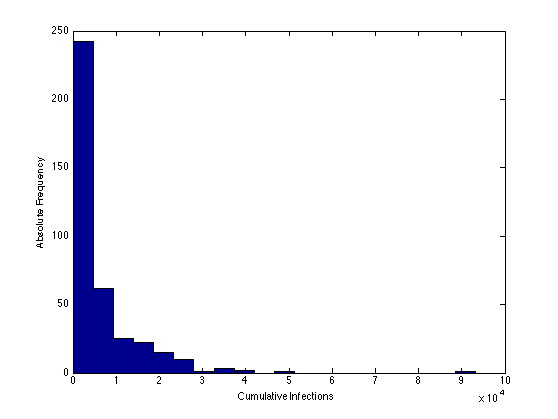
\includegraphics[width=7cm]{influ2}
\caption{sdlhfa}
\label{Histo}
\end{figure}

\begin{figure}
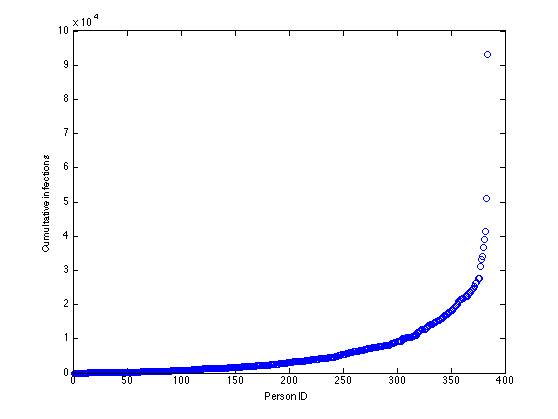
\includegraphics[width=7cm]{influ1}
\caption{sdlhfa}
\label{Sorted}
\end{figure}

Figure \ref{Histo} is a simple histogramm, that shows that the vast majority of people has only a small cumulative infection value. Whereas we see in Figure \ref{sorted} (which again plots the cumultative infection, sorted from small to large), that there are only a few with a very large cumultative infection value. \\

We can even go one step further and try to estimate the importance of those influentials on all infections that occur in total. In order to do so, we sort the people after their importance (defined as above). We then calculate the amout of infections conditioned that only the m least important person have been involved in the spreading process (1 $\le$ m $\le$ 384).\\
For instance, $m=384$ implies all infections that occured, when only the last (therefore most important) person has been excluded.\\
\\
Given these results, we get that 94\% of all infections, happen in the runs where the 1\%-quantile of the most important people (in our case 4) have contributed (ie. were not excluced). This again indicates their importance.

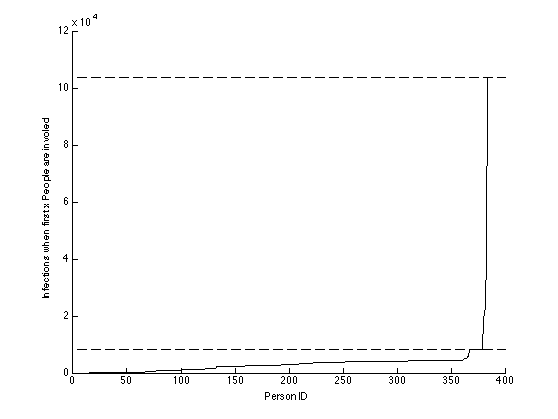
\includegraphics[width=7cm]{influ3}


According to the paper "Talk of the Network: A Complex Systems Look at the Underlying Process of Word-of-Mouth" the importance of influential often over-estimated. Our simulation contradicts this statement. 

Reasons might be, that our networt is a) of relative small size, b) we kinda cut the network. We only look at mutualfriends ,but not all friends of friends. So we might underestimated some people. 

\subsubsection{Determine influentials}